\chapter{Extension to Vector-Valued It\^o Processes}\label{chap13}

\begin{defi*}
Let\pageoriginale $(\Omega,\mathscr{F},P)$ be a probability space and
$(\mathscr{F}_{t})$ an increasing family of sub $\sigma$-algebras of
$\mathscr{F}$. Suppose further that 
\begin{equation*}
a:[0,\infty)\times \Omega\to S^{d}_{+}\tag{i}
\end{equation*}
is a probability measurable, bounded function taking values in the
class of all symmetric positive semi-definite $d\times d$ matrices,
with real entries;
\begin{equation*}
b:[0,\infty)\times \Omega\to \mathbb{R}^{d}\tag{ii}
\end{equation*}
is a progressively measurable, bounded function;
\begin{equation*}
X:[0,\infty)\times\Omega\to \mathbb{R}^{d}\tag{iii}
\end{equation*}
is progressively measurable, right continuous for every $w$ and
continuous almost everywhere $(P)$;
\begin{align*}
Z(t,\cdot) &= \exp[\langle \theta, X(t,\cdot)\rangle
  -\int\limits^{t}_{0}\langle \theta,b(s,\cdot)\rangle ds\\
&\q
  -\frac{1}{2}\int\limits^{t}_{0}\langle\theta,\ a(s,\cdot)\theta\rangle
  ds]\tag{iv}
\end{align*}
is a martingale for each $\theta\in \mathbb{R}^{d}$, where
$$
\langle x,y\rangle=x_{1}y_{1}+\cdots+x_{d}y_{d},\ x,\ y\in R^{d}.
$$

Then $X$ is called an It\^o process corresponding to the parameters
$b$ and $a$, and we write $X\in I[b,a]$
\end{defi*}

\begin{note*}
\begin{enumerate}
\item $Z(t,w)$ is a real valued function.

\item $b$ is progressively measurable if and only if each $b_{i}$ is
  progressively measurable.

\item $a$\pageoriginale is progressively measurable if and only if
  each $a_{ij}$ is so.
\end{enumerate}
\end{note*}

\setcounter{exercise}{0}
\begin{exercise}\label{chap13-exer1}
If $X\in I[b,a]$, then show that
\begin{gather*}
X_{i}\in I[b_{i},a_{ii}],\tag{i}\\
Y=\sum\limits^{d}_{i=1}\theta_{i}X_{i}\in I[\langle \theta,b\rangle,
  \langle \theta,a\theta\rangle],\tag{ii}
\end{gather*}
where
$$
\theta=(\theta_{1},\ldots,\theta_{d}).
$$
(Hint: (ii) (i). To prove (ii) appeal to the definition).
\end{exercise}

\begin{remark*}
If $X$ has a multivariate normal distribution with mean $\mu$ and
covariance $(\rho_{ij})$, then $Y=\langle \theta,X\rangle$ has also a
normal distribution with mean $\langle\theta,\mu\rangle$ and variance
$\langle \theta,\rho\theta\rangle$. Note the analogy with the above
exercise. This analogy explains why at times $b$ is referred to as the
``mean'' and $a$ as the ``covariance''.
\end{remark*}

\begin{exercise}\label{chap13-exer2}
If $\{\beta(t):t\geq 0\}$ is a $d$-dimensional Brownian motion, then
$\beta(t,w)\in I[0,I]$ where $I=d\times d$ identity matrix.

As before one can show that
$Y(t,\cdot)=X(t,\cdot)-\int\limits^{t}_{0}b(s,w)ds$ is an It\^o
process with parameters $0$ and $a$.
\end{exercise}

\begin{defi*}
Let $X$ be a $d$-dimensional Ito
process. $\sigma=(\sigma_{1},\ldots,\sigma_{d})$ a $d$-dimensional
progressively measurable function such that
$$
E\left(\int\limits^{t}_{0}\langle
\sigma(s,\cdot),\sigma(s,\cdot)\rangle> ds\right)
$$
is finite or, equivalently,
$$
E\left(\int\limits^{t}_{0}\sigma^{2}_{i}(s,\cdot)ds\right)<\infty,\q
(i=1,2,\ldots d).
$$\pageoriginale

Then by definition
$$
\int\limits^{t}_{0}\langle \sigma(s,\cdot),dX(s,\cdot)\rangle
=\sum\limits^{d}_{i=1}\int\limits^{t}_{0}\sigma_{i}(s,\cdot)dX_{i}(s,\cdot).
$$
\end{defi*}

\begin{prop*}
Let $X$ be a $d$-dimensional It\^o process $X\in I[b,a]$ and let
$\sigma$ be progressively measurable and bounded. If
$$
\xi_{i}(t,\cdot)=\int\limits^{t}_{0}\sigma_{i}dX_{i}(s,\cdot),
$$
then
$$
\xi=(\xi_{1},\ldots,\xi_{d})\in I[B,A],
$$
where
$$
B=(\sigma_{1}b_{1},\ldots,\sigma_{d}b_{d})\q\text{and}\q
A_{ij}=\sigma_{i}\sigma_{j}a_{ij}. 
$$
\end{prop*}

\begin{proof}
\begin{enumerate}
\renewcommand{\theenumi}{\roman{enumi}}
\renewcommand{\labelenumi}{(\theenumi)}
\item Clearly $A_{ij}$ is progressively measurable and bounded. 

Since  $a\in S^{d}_{+}$, $A\in S^{d}_{+}$.

\item Again $B$ is progressively measurable and bounded.

\item Since $\sigma$ is bounded, each $\xi_{i}(t,\cdot)$ is an It\^o
  process; hence $\xi$ is progressively measurable, right continuous,
  continuous almost everywhere $(P)$. It only remains to verify the
  martingale condition.
\end{enumerate}

\setcounter{step}{0}
\begin{step}%1
Let $\theta=(\theta_{1},\ldots,\theta_{d})\in \mathbb{R}^{d}$. By
hypothesis,
\begin{align*}
&E(\exp[(\theta_{1}X_{1}+\cdots+\theta_{d}X_{d})|^{t}_{s}\cdots\int\limits^{t}_{s}(\theta_{1}b_{1}+\cdots+\theta_{d}b_{d})du\tag{*}\\
&\q
    {}-\frac{1}{2}\int\limits^{t}_{0}\sum\theta_{i}\theta_{j}a_{ij}ds]|\mathscr{F}_{s})=1. 
\end{align*}

Assume\pageoriginale that each $\sigma_{i}$ is constant on $[s,t]$,
$\sigma_{i}=\sigma_{i}(w)$ and $\mathscr{F}_{s}$-measurable. Then (*)
remains true if $\theta_{i}$ are replaced by $\theta_{i}\theta_{i}(w)$
and since $\sigma_{i}$'s are constant over $[s,t]$, we get
\begin{align*}
& E(\exp[\int\limits^{t}_{0}\sum^{d}_{i=1}\theta_{i}\sigma_{i}(s,\cdot)dX_{i}(s,\cdot)-\int\limits^{t}_{0}\theta_{i}b_{i}\sigma_{i}(s,\cdot)ds\\
&\qq -\frac{1}{2}\int\limits^{t}_{0}\sum
    \theta_{i}\theta_{j}\sigma_{i}(s,\cdot)\sigma_{j}(s,\cdot)a_{ij}ds]|_{s})\\
&
  \exp\left[\int\limits^{s}_{0}\sum^{d}_{i=1}\theta_{i}\sigma_{i}(s,\cdot)dX_{i}(s,\cdot)-\int\limits^{s}_{0}\langle
    \theta,B\rangle du-1\int\limits^{s}_{0}\langle
    \theta,A\theta\rangle du\right].
\end{align*}
\end{step}

\begin{step}%2
Let each $\sigma_{i}$ be a simple function.
\begin{figure}[H]
\centering
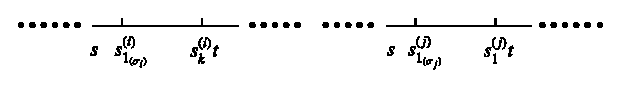
\includegraphics{figure/fig10.eps}
\end{figure}

By considering finer partitions we may assume that each $\sigma_{i}$
is a step function,
\begin{figure}[H]
\centering
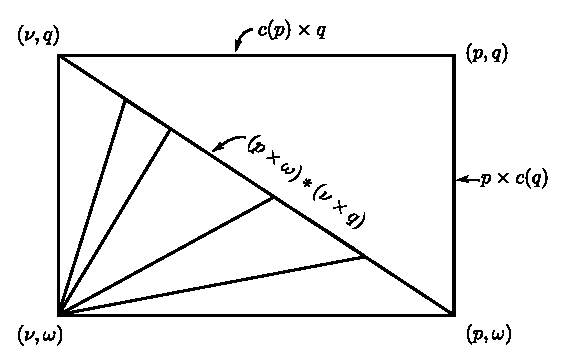
\includegraphics{figure/fig11.eps}
\end{figure}
\noindent
i.e.\@ there exist points $s_{0}$, $s_{1}$,
$s_{2},\ldots,s_{n},s=s_{0}<s_{1}<\ldots<s_{n+1}=t$, such that on
$[s_{j},s_{j+1})$ each $\sigma_{i}$ is a constant and
  ${}_{s_{j}}$-measurable. Then (**) holds if we use the fact that if
  $\mathscr{C}_{1}\supset \mathscr{C}_{2}$.
$$
E(E(f|\mathscr{C}_{1})|\mathscr{C}_{2})=E(f|\mathscr{C}_{2}).
$$
\end{step}

\begin{step}%3
Let $\sigma$ be bounded, $|\sigma|\leq C$. Let $(\sigma^{(n)})$ be a
sequence of simple functions approximating $\sigma$ as in Lemma
\ref{chap11-lem3}. (**) is true if $\sigma_{i}$ is\pageoriginale
replaced by $\sigma^{(n)}_{i}$ for each $n$. A simple verification
shows that the expression $Z_{n}(t,\cdot)$, in the parenthes is on the
left side of (**) with $\sigma_{i}$ replaced by $\sigma^{(n)}_{i}$,
converges to
\begin{gather*}
Z(t,\cdot)=\\
=\Exp\Big(\int\limits^{t}_{0}\sum_{i}\theta_{i}\sigma_{i}(s,\cdot)ds-\int\limits^{t}_{0}\sum_{i}\theta_{i}b_{i}\sigma_{i}(s,\cdot)ds-\\
-\frac{1}{2}\int\limits^{t}_{0}\sum_{i,j}\theta_{i}\theta_{j}\sigma_{i}\sigma_{j}a_{ij}ds\Big)
\end{gather*}
as $n\to \infty$ in probability. Since $Z_{n}(t,\cdot)$ is a
martingale and the functions $\sigma_{i}$, $\sigma_{j}$, $a$ are all
bounded,
$$
\sup\limits_{n}E(Z_{n}(t,\cdot))<\infty.
$$
\end{step}

This proves that $Z(t,\cdot)$ is a martingale.
\end{proof}

\begin{coro*}
With the hypothesis as in the above proposition define
$$
Z(t)=\int\limits^{t}_{0}\langle \sigma(s,\cdot),dX(s,\cdot)\rangle.
$$

Then
$$
Z(t,\cdot)\in I[\langle \sigma,b\rangle, \sigma a\sigma^{*}]
$$
where $\sigma^{*}$ is the transpose of $\sigma$.
\end{coro*}

\begin{proof}
$Z(t,\cdot)=\xi_{1}(t,\cdot)+\cdots+\xi_{d}(t,\cdot)$.
\end{proof}

\begin{defi*}
Let $\sigma(s,w)=(\sigma_{ij}(s,w))$ be a $n\times d$ matrix of
progressively measurable functions with
$$
E\left(\int\limits^{t}_{0}\sigma^{2}_{ij}(s,\cdot)ds\right)<\infty.
$$

If\pageoriginale $X$ is a $d$-dimensional It\^o process, we define
$$
\left(\int\limits^{t}_{0}\sigma(s,\cdot)dX(s,\cdot)\right)_{i}=\sum\limits^{d}_{j=1}\int\limits^{t}_{0}\sigma_{ij}(s,\cdot)dX_{j}(s,\cdot).
$$
\end{defi*}

\begin{exercise}\label{chap13-exer3}
Let
$$
Z(t,w)=\int\limits^{t}_{0}\sigma(s,\cdot)dY(s,\cdot),
$$
where $Y\in I[0,a]$ is a $d$-dimensional It\^o process and $\sigma$ is
as in the above definition. Show that
$$
Z(t,\cdot)\in I[0,\sigma a\sigma^{*}]
$$
is an $n$-dimensional Ito process, (assume that $\sigma$ is bounded).
\end{exercise}

\begin{exercise}\label{chap13-exer4}
Verify that
$$
E(|Z(t)|^{2})=E\left(\int\limits^{t}_{0}\tr(\sigma
a\sigma^{*})ds\right).
$$
\end{exercise}

\begin{exercise}\label{chap13-exer5}
Do exercise 3 with the assumption that $\sigma a\sigma^{*}$ is bounded.
\end{exercise}

\begin{exercise}\label{chap13-exer6}
State and prove a change of variable formula for stochastic integrals
in the case of several dimensions.

\noindent
(Hint:~ For the proof, use the change of variable formula in the one
dimensional case and $d(X+Y)=dX+dY$).
\end{exercise}
